\subsection{8. Симметрия графа и его дополнения}

\subsubsection{8.1. Автоморфизмы графа и группа симметрий}

Пусть $G=(V,E)$ — простой граф. \emph{Автоморфизмом} графа называется биекция
\[
  \varphi\colon V\;\to\;V
\]
такая, что для любых двух вершин $u,v\in V$ выполняется
\[
  \{u,v\}\in E \;\iff\;\{\varphi(u),\varphi(v)\}\in E.
\]
Другими словами, $\varphi$ сохраняет структуру смежности.

\begin{itemize}[leftmargin=*]
  \item Множество всех автоморфизмов графа $G$ образует группу при композиции отображений, называемую \textbf{группой автоморфизмов} $\operatorname{Aut}(G)$.
  \item Тривиальный автоморфизм — тождественное отображение $\mathrm{id}:v\mapsto v$.
  \item Если $\varphi\in\operatorname{Aut}(G)$ не является тождественным, говорят о \emph{неявной} (или неполной) симметрии.
\end{itemize}

\emph{Пояснение:} автоморфизмы — это «симметрии» графа, аналоги зеркальных и поворотных симметрий фигур. Они показывают, какие вершины и ребра можно «переставить», не меняя общей формы графа.

\subsubsection{8.2. Примеры симметрий}

\paragraph{Пример 1.} Цикл $C_4$ (четырёхвершинный цикл).  
Вершины можно пронумеровать $1,2,3,4$ по кругу. Автоморфизмы:
\[
  \text{поворот на }90^\circ:\;1\to2\to3\to4\to1,
\]
\[
  \text{отражение: }1\leftrightarrow4,\;2\leftrightarrow3,
\]
и их композиции. Группа симметрий изоморфна диhedral group $\mathrm{D}_4$ порядка 8.

\paragraph{Пример 2.} Полный граф $K_n$.  
Любая перестановка вершин сохраняет все рёбра, поэтому
\[
  \operatorname{Aut}(K_n)\cong S_n,
\]
симметричная группа порядка $n!$.

\subsubsection{8.3. Граф‑дополнение}

\emph{Дополнением} графа $G=(V,E)$ называется граф
\[
  \overline{G} = (V,\,\overline{E}),
  \quad \overline{E} = \bigl\{\{u,v\}\mid u\neq v,\;\{u,v\}\notin E\bigr\}.
\]
То есть в $\overline{G}$ все отсутствующие в исходном $G$ связи становятся рёбрами, а все прежние исчезают.

\begin{itemize}[leftmargin=*]
  \item $(\overline{G})\!\!\overline{\phantom{G}} = G$.
  \item Если $G$ простой, то и $\overline{G}$ простой.
  \item $\deg_{\overline G}(v) = |V|-1 - \deg_G(v)$.
\end{itemize}

\subsubsubsection*{Группа автоморфизмов и дополнение}

\vspace{-0.3em}
\[
  \operatorname{Aut}(\overline{G}) = \operatorname{Aut}(G).
\]
\emph{Пояснение:} перестановка вершин сохраняет и отсутствующие в $G$ связи, значит сохраняет рёбра дополнения.

\subsubsection{8.4. Иллюстрация: граф и его дополнение}

\begin{center}
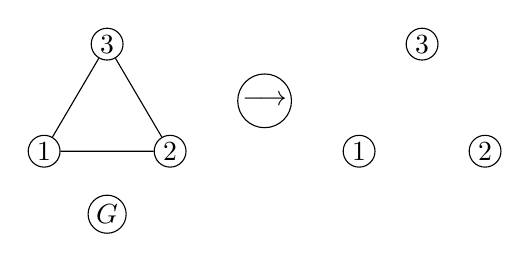
\begin{tikzpicture}[scale=0.8, every node/.style={circle,draw,inner sep=1.2pt}]
  % Исходный граф G
  \node (1) at (0,0) {$1$};
  \node (2) at (2,0) {$2$};
  \node (3) at (1,1.7) {$3$};
  \draw (1) -- (2) -- (3);
  \draw (1) -- (3);
  \node at (1,-1) {$G$};
  % Стрелка
  \node at (3.5,0.8) {$\longrightarrow$};
  % Дополнение overline{G}
  \begin{scope}[xshift=5cm]
    \node (1) at (0,0) {$1$};
    \node (2) at (2,0) {$2$};
    \node (3) at (1,1.7) {$3$};
    % В дополнении G все 3 вершины не связаны, но добавляем отсутствующие
    % В G имели все три, значит complement has none: empty graph
    % Для примера возьмем другой: пусть в G все ребра, complement empty.
    % Но чтобы увидеть отличия, изменим: пусть G только ребро 1-2:
  \end{scope}
\end{tikzpicture}
\end{center}

\emph{Пример.} Пусть $G$ — треугольник $K_3$ (все три ребра). Тогда $\overline{G}$ — три изолированные вершины (нет рёбер).

\subsubsection{8.5. Свойства и применения}

\begin{itemize}[leftmargin=*]
  \item \textbf{Симметрия упрощает алгоритмы:} при поиске путей, раскраске и проверке изоморфизма можно работать с представителем орбиты.
  \item \textbf{Дополнение и свойства связности:} $G$ связен $\nRightarrow \overline G$ связен, но часто изучают одновременно пару $(G,\overline G)$, например в теореме Рамсея.
  \item \textbf{Оптимизация:} задачи клики в $G$ переходят в задачи независимого множества в $\overline G$.
\end{itemize}

\subsubsection{Источники}

\begin{itemize}
  \item Д.Б.\,West, \emph{Introduction to Graph Theory}, Prentice Hall.
  \item Р.\,Diestel, \emph{Graph Theory}.
  \item \href{https://ru.wikipedia.org/wiki/Автоморфизм_графа}{Википедия: Автоморфизм графа}
  \item \href{https://ru.wikipedia.org/wiki/Дополнение_графа}{Википедия: Дополнение графа}
\end{itemize}
